\chapter*{Experiment 4 - Thermistor}
\addcontentsline{toc}{chapter}{Experiment 4 - Thermistor}
We wire up the experiment as shown in the diagram fig:~\ref{fig:exp4_thermistor}. And upload the sketch code in the next section on page:~\pageref{sketch:exp4}.

%
\begin{figure}[ht]
	\centering
	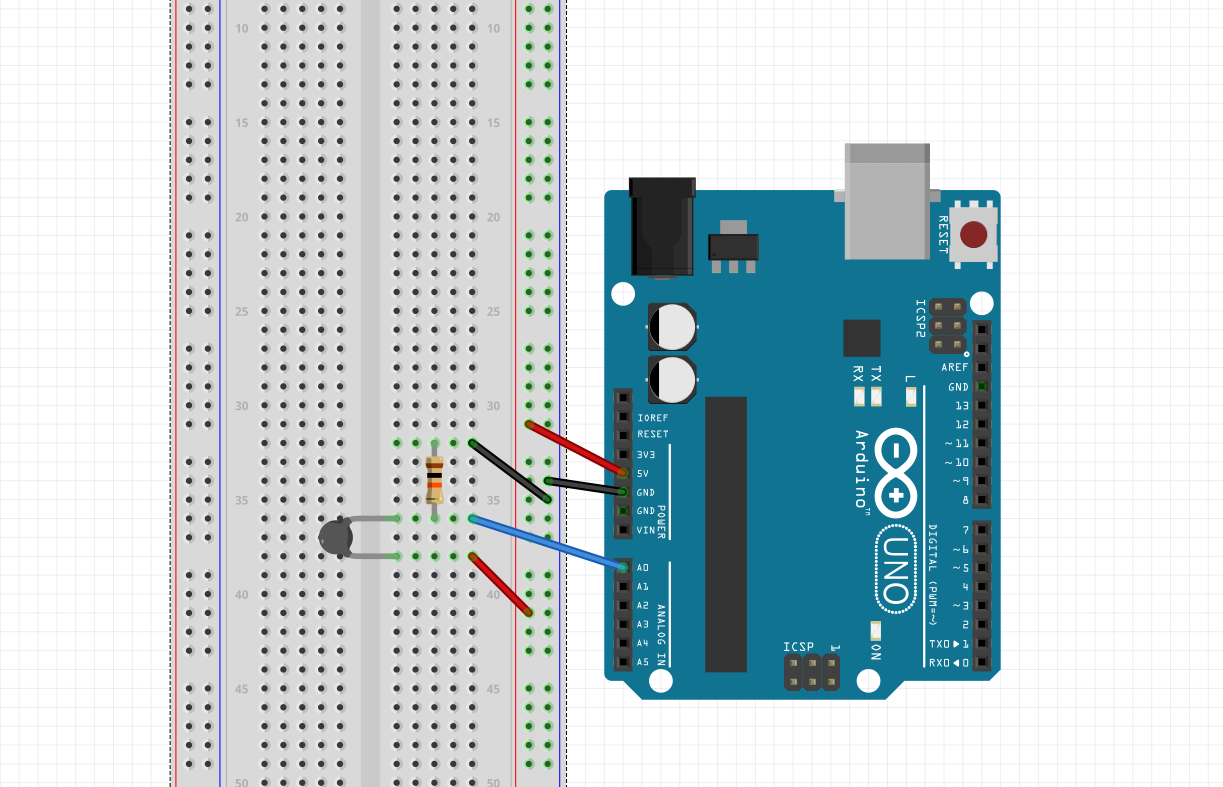
\includegraphics[width=12cm]{images/19}
	\caption{Read a Thermistor Value}
	\label{fig:exp4_thermistor}
\end{figure}
%

The thermistor is an electrical resistor whose resistance is greatly reduced by heating. Its often used for measurement and control applications. The following graph fig:~\ref{fig:exp4_thermistor_plot} on page:~\pageref{fig:exp4_thermistor_plot}. demonstrates the fall of resistance as the temperature rises.

To view the values being read from the thermistor, simply open the Arduino serial monitor.

%
\begin{figure}[ht]
	\centering
	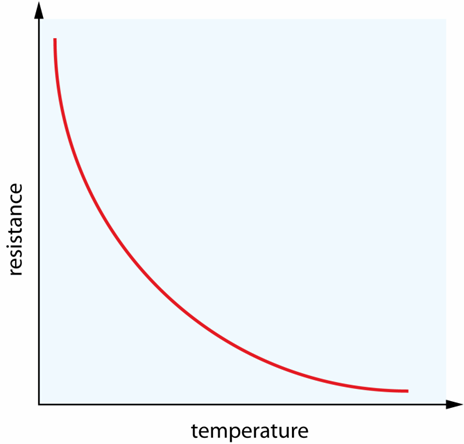
\includegraphics[width=12cm]{images/20}
	\caption{Thermistor Plot: Resistance vs Temperature}
	\label{fig:exp4_thermistor_plot}
\end{figure}
%

\newpage
\section*{Sketch Code}
\label{sketch:exp4}
\begin{lstlisting}
/*
Sample code to work with a Thermistor

Author: David Kirwan
Licence: Apache 2.0
*/

int sensorPin = A0;
int sensorValue = 0;

void setup() {
  // declare the ledPin as an OUTPUT:
  Serial.begin(9600);
  pinMode(sensorPin, INPUT);
}

void loop() {
  // read the value from the sensor:
  sensorValue = analogRead(sensorPin);
  Serial.println(sensorValue);
  delay(sensorValue);
}
\end{lstlisting}